\documentclass[a4paper]{exam}

\usepackage{geometry}
\usepackage{graphicx}
\usepackage{hyperref}
\graphicspath{{images/}}
\usepackage{tikz}
\usetikzlibrary{arrows.meta, positioning}
% \usepackage{algorithm}
\usepackage{algorithmic}

\printanswers
\addpoints

\title{Homework Assignment 2}
\author{CS/CE 412/471 Algorithms: Design and Analysis, Spring 2025}
\date{\numquestions\ problems, \numpoints\ points}

\qformat{{\large\bf \thequestion. \thequestiontitle}\hfill[\totalpoints\ points]}
\boxedpoints
\newcommand\heading[1]{\subsubsection*{#1}}

\begin{document}
\maketitle
\thispagestyle{empty}

\includegraphics[trim=0 2cm 0 0cm, clip, width=\textwidth]{title}
\begin{questions}
  

\titledquestion{Introduction to Epidemiology}

  You are given a set of nodes representing villages and mountains. Some villages are initially infected, and others are healthy. Villages are connected by undirected paths, which define how the disease can potentially spread. There is a path between any two nodes, but the disease cannot cross a mountain. That is, a mountain is a special type of node through which the disease cannot enter or pass.
  
Each day, the disease spreads from an infected village to its directly connected healthy villages. We are interested to:
\begin{itemize}
\item Visualize the graph.
\item Simulate the spread of the disease over time.
\item Compute the minimum number of days required to infect all reachable healthy villages.
\item Identify the healthy villages that cannot be infected (due to mountain barriers).
\end{itemize}

\heading{Input Format}

The first line of the input contains two integers, $n$ and $m$, the numbers of nodes and edges respectively, where $n-1\le m\le \frac{n(n-1)}{2}$.

The next $m$ lines each contain two integers, $u$ and $v$, indicating an edge between vertex $u$ and vertex $v$ where $0 le u,n < n$.

The next line contains two integers $p$ and $q$, the number of mountains and initially infected villages respectively, where $(1\le p,q \le n)$ and $2\le p+q \le n$.

The next line contains $p$ integers $a_1\ a_2\ a_3\ldots a_p$ where each $0 \le a_i< n$ indicates a mountain.

The next line contains $q$ integers $b_1\ b_2\ b_3\ldots b_q$ where each $0 \le b_j< n$ indicates an initially infected village.

It is guaranteed that $a_i\ne b_j$ for all valid values of $i$ and $j$,

\heading{Output Format}

The first line of the output should contain a single integer denoting the minimum number of days to infect all reachable healthy villages. Output 0 if all reachable villages are already infected.

The second line of the output contains the nodes that represent the healthy villages that cannot be infected. Output 0 if all healthy villages can get infected.

\heading{Sample}
\begin{minipage}{.2\textwidth}
\begin{tabular}{|l|l|}
  \hline
  Input & Output\\\hline
7 6 & 2 \\
1 2 & 5 6 7\\
2 3 & \\
3 4 & \\
4 5 & \\
5 6 & \\
8 7 & \\
1 1 & \\
4 & \\
1 & \\\hline
\end{tabular}
\end{minipage}
\begin{minipage}{.75\textwidth}
The input describes a graph with $n=7$ nodes and $m=6$ edges. The next 6 lines describe the edges. There are $p=1$ mountain nodes and $q=1$ initially infected village nodes. The $p=1$ nodes representing mountains are: $4$. The $q=1$ nodes representing initially infected villages are: $1$.

The output declares a minimum of 2 days for the maximal spread of the disease. On Day 1, the disease spreads from node 1 to node 2. On Day 2, it spreads from node 2 to node 3. It cannot spread further as it is blocked by the mountain at 4. The output declares that the villages $5, 6, 7$ do not get infected.
\end{minipage}

\heading{Tasks}

\begin{parts}
\part[5] Design a linear-time algorithm to simulate the spread. That is, ensure your solution runs in $\mathcal{O}(n + m)$ time, where $n$ is the number of nodes and $m$ is the number of edges. Describe below any considerations, e.g. appropriate data structures, to ensure the linear run time.
  \begin{solution}
    
  \end{solution}
\part[5] Submit files, \texttt{disease.in} and \texttt{disease.py}, where the former contains input and the latter reads the input and implements your algorithm on it to produce the output. You may design any reasonable input. 
\part[5] Submit an animation, \texttt{disease.mp4}, which simulates the spread of the disease on your graph from above. The last frame should include the output of your program.
\end{parts}


%\maketitle
\titledquestion{Pakistan Trip Planning}[10]

  For this problem, we will study the road network of Pakistan to construct a graph modeling the roads between at least 12 cities, listed below, and implement an All-Pairs Shortest Path Algorithm (e.g., Floyd-Warshall) to find the shortest road distance between any pair of cities. You will write a program that visualizes the network, and interactively displays the shortest road distance between two input cities.

  The cities include the capital cities of each province/region:
  \begin{itemize}
    \item Islamabad (Capital Territory)
    \item Lahore (Punjab)
    \item Karachi (Sindh)
    \item Peshawar (Khyber Pakhtunkhwa)
    \item Quetta (Balochistan)
    \item Muzaffarabad (Azad Jammu \& Kashmir)
    \item Gilgit (Gilgit-Baltistan)
    \item At least five other major cities of your choice.
  \end{itemize}

  \begin{parts}
  \part[5] Submit a file, \texttt{roads.py}, that hard codes the graph, visualizes it, applies your chosen all-pairs shortest path algorithm on it and stores the distances, and handles interactive queries (case-insensitive and handling invalid input).
  \part[5] Include below any notes on your approach, cities used, and assumptions.
    \begin{solution}
      So, one assumption that I did for the hardcoded data was to only include weights between those cities between which a direct road exists and not a road which goes through multiple cities instead first. This is to just make the graph a bit small otherwise it would appear extremely cluttered because technically speaking a road exists between all cities in the data set. This required a lot of Google searches so I cannot guarantee that my data is completely correct but logically it works for the question. Extra cities that were used included Gwadar, Nawabshah, Hyderabad, and Rawalpindi.
    \end{solution}
  \part[5] Submit a short demo video (no longer than 5 minutes), \texttt{roads.mp4}, of a run of your program. The video should include the graph visualization, interaction with the user, and commentary by you including details of the algorithm, visualization, and interaction. Make sure that the visualization highlights any selected shortest route.
  \end{parts}


\titledquestion{Greedy Bucket}

  Figure \ref{fig:bucket} presents the Bucket Algorithm (Algorithm A) and illustrates a few steps of its dry run on an unweighted and undirected graph in which the bucket is represented by the purple colored area. The algorithm appears to useful to detect connected components in the graph. However, with slight modifications, it can do a lot more!

  Figure \ref{fig:bucketspan} presents Algorithm B which modifies Algorithm A to output a tree containing connected vertices. Such a tree is called the \textit{spanning tree}. Formally, ``a spanning tree $T$ of an undirected graph $G$ is a subgraph that is a tree which includes all of the vertices of $G$. In general, a graph may have several spanning trees, but a graph that is not connected will not contain a spanning tree $\ldots$ [rather a] spanning forest.''\footnote{\url{https://en.wikipedia.org/wiki/Spanning_tree}}
  
  \begin{figure}
    \begin{center}
    \begin{minipage}{.8\textwidth}
    \textbf{Algorithm A: The Bucket Algorithm}\\
    \underline{Input:} Graph $G = (V, E)$\\
    \underline{Output:} Bucket $B \subseteq V$ (a set of vertices)

    \begin{enumerate}
    \item Choose any vertex $x \in V$
    \item Initialize Bucket $B \leftarrow x$
    \item While there exists an edge $(u, v) \in E$ such that $u \in B$ and $v \not\in B$:
      \begin{enumerate}
      \item Add vertex $v$ to $B$
      \end{enumerate}
    \end{enumerate}
  \end{minipage}\\[5pt]

    \rule{300pt}{.5pt}\\
    \includegraphics[scale=0.6]{a}
    \includegraphics[scale=0.6]{b}
    \includegraphics[scale=0.6]{c}
    \includegraphics[scale=0.6]{d}      
  \end{center}
  \caption{The bucket algorithm (top) and a visualization (bottom) of a run of the algorithm on an unweighted and undirected graph. The \textit{bucket} is represented by the purple colored area. It expands from one step to the next.}
    \label{fig:bucket}
  \end{figure}
  \begin{figure}
    \begin{center}
    \begin{minipage}{.8\textwidth}
\textbf{Algorithm B: Bucket Algorithm with Spanning Tree}\\
\underline{Input:} Graph $G = (V, E)$ represented as an adjacency matrix\\
\underline{Output:} Spanning tree $T$

\begin{enumerate}
    \item Choose any vertex $x \in V$
    \item Initialize Bucket $B \leftarrow x$, Tree $T \leftarrow \emptyset$
    \item While there exists an edge $(u, v) \in E$ such that $u \in B$ and $v \not\in B$:
    \begin{enumerate}
        \item Add vertex $v$ to $B$
        \item Add edge $(u, v)$ to $T$
    \end{enumerate}
    \item Return $T$
\end{enumerate}      
    \end{minipage}
  \end{center}
  \caption{The bucket algorithm from Figure \ref{fig:bucket} is modified to compute a spanning tree.}
    \label{fig:bucketspan}
  \end{figure}

  \begin{parts}
  \part[5]  Modify Algorithm B to operate on a \textit{weighted} undirected graph and output its Minimum Spanning Tree i.e. a spanning tree that connects all the vertices with the least possible sum of edge weights. Call this Algorithm C.\\
    (Hint: be greedy in step 3b).
    \begin{solution}
      \textbf{Algorithm C: Bucket Algorithm with Minimum Spanning Tree}\\
      \underline{Input:} Graph $G = (V, E)$ represented as an adjacency matrix\\
      \underline{Output:} Minimum spanning tree $T$

      \begin{enumerate}
          \item Choose any vertex $x \in V$
          \item Initialize Bucket $B \leftarrow x$, Tree $T \leftarrow \emptyset$
          \item While there exists an edge $(u, v, w) \in E$ such that $u \in B$ and $v \not\in B$:
          \begin{enumerate}
              \item Find the edge $(u, v, w)$ with the minimum weight $w$
              \item Add vertex $v$ to $B$
              \item Add edge $(u, v, w)$ to $T$
          \end{enumerate}
          \item Return $T$
      \end{enumerate}      
    \end{solution}
  \part[5] For Algorithm C that you developed above, visualize its run on the graph below starting from vertex $a$. Highlight the bucket and the minimum spanning tree edges at every step to clearly show how they grow (as shown in the sample dry run for Algorithm A).
    \begin{solution}\null\\
    \includegraphics[scale=0.4]{e}
    \includegraphics[scale=0.2]{Q3/images3b/3b1}
    \includegraphics[scale=0.2]{Q3/images3b/3b2}\\
    \includegraphics[scale=0.2]{Q3/images3b/3b3}
    \includegraphics[scale=0.2]{Q3/images3b/3b4}
    \includegraphics[scale=0.2]{Q3/images3b/3b5}
    \includegraphics[scale=0.2]{Q3/images3b/3b6}
    \includegraphics[scale=0.2]{Q3/images3b/3b7}
    \includegraphics[scale=0.2]{Q3/images3b/3b8}
    \includegraphics[scale=0.2]{Q3/images3b/3b9}
    \includegraphics[scale=0.2]{Q3/images3b/3b10}
    \includegraphics[scale=0.25]{Q3/images3b/3b11}

    \end{solution}
  \part[5] Derive the time complexity of Algorithm C.
    \begin{solution}
      The time complexity of Algorithm B is $\mathcal{O}(n + m)$, where $n$ is the number of vertices and $m$ is the number of edges. The time complexity of Algorithm C is also $\mathcal{O}(n^2)$, as we are iterating over the edges of each vertex. Since the worst case is when the graph is dense (each vertex is connected to every other vertex), we can say that the time complexity of Algorithm C is $\mathcal{O}(n^2)$.
    \end{solution}
  \part[5] Now let’s design another algorithm, where now we \textit{remove} certain edges frmo $G$ such that the resulting graph is a Minimum Spanning Tree. Let’s call this Algorithm D.\\
    Note that while removing edges, we need to make sure the graph stays connected! To check connectivity use Algorithm A.
    \begin{solution}
      \textbf{Algorithm D:Remove Edges to form Minimum Spanning Tree}\\
      \underline{Input:} Graph $G = (V, E)$ represented as an adjacency matrix\\
      \underline{Output:} Minimum spanning tree $T$

      \begin{enumerate}
        \item Initialize EdgeSet $E \leftarrow E$.
        \item Sort all edges in $E$ in non-decreasing order of their weights.
        \item Initialize TreeSet $T \leftarrow \emptyset$.
        \item For each edge $(u, v, w)$ in sorted order:
        \begin{enumerate}
            \item If adding edge $(u, v, w)$ to $T$ does not create a cycle:
            \begin{enumerate}
                \item Add edge $(u, v, w)$ to $T$.
            \end{enumerate}
        \end{enumerate}
        \item Let removeSet $R \leftarrow E - T$ (edges not included in the MST).
        \item For each edge $(u, v, w)$ in $R$:
        \begin{enumerate}
            \item Remove edge $(u, v, w)$ from $G$.
        \end{enumerate}
        \item Return $T$.
    \end{enumerate}
    
    \end{solution}
  \part[5] For Algorithm D that you developed above, visualize its run on the graph below starting from vertex $a$. Highlight the edges you are deleting at every step to clearly show how the graph shrinks into an MST.
    \begin{solution}\null\\
    Shown is the dry run of the algorithm that will form the MST, with the orange vertices/edges depicting the ones that will be added to the MST. The final graph has the edges (highlighted in red) that will re removed from G.\\  
    \includegraphics[scale=0.4]{e}
    \includegraphics[scale=0.25]{Q3/images3e/3e2}
    \includegraphics[scale=0.25]{Q3/images3e/3e3}\\
    \includegraphics[scale=0.25]{Q3/images3e/3e4}
    \includegraphics[scale=0.25]{Q3/images3e/3e5}
    \includegraphics[scale=0.25]{Q3/images3e/3e6}\\
    \includegraphics[scale=0.25]{Q3/images3e/3e7}
    \includegraphics[scale=0.2]{Q3/images3e/3e8}
    \includegraphics[scale=0.25]{Q3/images3e/3e9}\\
    \includegraphics[scale=0.25]{Q3/images3e/3e10}
    \includegraphics[scale=0.6]{Q3/images3e/3e1}
    \includegraphics[scale=0.25]{Q3/images3e/3e11}\\
    \includegraphics[scale=0.25]{Q3/images3e/3e12.jpeg}
    \end{solution}For Algorithm D that you’ve designed in part c), dry run it on the graph below. 
  \part[5] Derive the time complexity of Algorithm D.
    \begin{solution}
      \\
      2. Sorting the edges takes $\mathcal{O}(V^2 \log V)$ time (since we are useing a matrix representation of G).\\
      4. Looping over all the edges takes $\mathcal{O}(V^2)$ time.\\
      4a. Checking for cycles takes $\mathcal{O}(V^2)$ time.\\
      5. Removing edges takes $\mathcal{O}(V^2)$ time.\\
      6. The final time complexity is $\mathcal{O}(V^2 \log V)$.

    \end{solution}
  \part[5]  Modify Algorithm B to output its \textit{Shortest Path Spanning Tree}. Unlike Minimum Spanning Tree (which minimizes the total weight of the tree), the Shortest Path Spanning Tree focuses on minimizing the distance from the root/starting vertex to each vertex.\\
    Hint: be greedy in step 3b). Call this Algorithm E.
    \begin{solution}
      \\
      \textbf{Algorithm E: Djikstra's Algorithm with Spanning Tree}\\
      \underline{Input:} Graph $G = (V, E)$ represented as an adjacency matrix\\
      \underline{Output:} Spanning tree $T$
    %   \begin{enumerate}
    %     \item Choose any vertex $x \in V$
    %     \item For all vertices $v \in V$, set $v.d \leftarrow \infty$ (distance to all vertices initially infinity)
    %     \item Set $x.d \leftarrow 0$ (distance to the root is zero)
    %     \item Initialize Bucket $B \leftarrow x$, Tree $T \leftarrow \emptyset$
    %     \item While there exists a vertex $u \in B$:
    %     \begin{enumerate}
    %       \item $u$ = node with the smallest distance among unvisited nodes
    %       \item For each neighbor $v$ of $u$:
    %       \begin{enumerate}
    %           \item If $d(v) > d(u) + w(u, v)$ (relaxation condition):
    %           \begin{enumerate}
    %               \item Update $d(v) \leftarrow d(u) + w(u, v)$
    %               % \item Add edge $(u, v)$ to $T$
    %           \end{enumerate}
    %           \item If $v$ is not in $B$ (it’s unvisited), add $v$ to $B$
    %       \end{enumerate}
    %       \item Remove vertex $u$ from $B$
    %   \end{enumerate}
    %   \item Return $T$
    % \end{enumerate}
    \textbf{Algorithm E: Dijkstra’s Algorithm with Shortest Path Spanning Tree (No Priority Queue)}\\
    \underline{Input:} Graph \( G = (V, E) \) represented as an adjacency matrix\\
    \underline{Output:} Shortest Path Spanning Tree \( T \)
    
    \begin{enumerate}
      \item Choose any vertex \( x \in V \)
      \item For all vertices \( v \in V \), set \( v.d \leftarrow \infty \) (distance to all vertices initially infinity)
      \item Set \( x.d \leftarrow 0 \) (distance to the root is zero)
      \item Initialize Bucket $B \leftarrow x$, Tree $T \leftarrow \emptyset$
      \item Initialize set S of visited vertices \( S \leftarrow \emptyset \)
      \item For all vertices, initialize \( pred(v) \leftarrow \emptyset \) (no predecessors at the start)
      \item While there exists an edge $(u, v) \in E$ such that $u \in B$ and $v \not\in B$:      
      \begin{enumerate}
        \item Select vertex \( u \) from \( B \) such that \( u.d \) is the smallest distance among $V - S$
        \item Add \( u \) to \( S \)
        \item For each neighbor \( v \) of \( u \) where \( v \notin B \):
        \begin{enumerate}
          \item If \( d(v) > d(u) + w(u, v) \), then:
          \begin{enumerate}
            \item Update \( d(v) \leftarrow d(u) + w(u, v) \) (relaxation)
            \item Add edge \( (u, v) \) to \( T \)
          \end{enumerate}
        \item Add \( v \) to \( B \)
        \end{enumerate}
      \end{enumerate}
      \item Return the Shortest Path Spanning Tree \( T \)
    \end{enumerate}
    
  
    \end{solution}
  \part For Algorithm E that you developed above, visualize its run on the graph below starting from vertex $a$. Highlight the bucket and the shortest path spanning tree edges at every step to clearly show how they grow (as shown in the sample dry run for Algorithm A).
    \begin{solution}\null\\
    \includegraphics[scale=0.4]{e}
    \includegraphics[scale=0.2]{Q3/images3g/3g1}
    \includegraphics[scale=0.2]{Q3/images3g/3g2}\\
    \includegraphics[scale=0.2]{Q3/images3g/3g3}
    \includegraphics[scale=0.2]{Q3/images3g/3g4}
    \includegraphics[scale=0.2]{Q3/images3g/3g5}\\
    \includegraphics[scale=0.2]{Q3/images3g/3g6}
    \includegraphics[scale=0.2]{Q3/images3g/3g7}
    \includegraphics[scale=0.2]{Q3/images3g/3g8}\\
    \includegraphics[scale=0.2]{Q3/images3g/3g9}
    \includegraphics[scale=0.2]{Q3/images3g/3g10}\\
    Notes:\\
    \begin{itemize}
      \item I have crossed out the nodes that are visited
      \item Node h is supposed to have $8,g$, not $8,f$.
    \end{itemize}
    \end{solution}
  \part Derive the time complexity of Algorithm E.
    \begin{solution}
      \\
      2. initialization takes takes $\mathcal{O}(V)$ time for setting up the distances and the predecessors.\\
      7. The while loop runs $\mathcal{O}(V)$ times.\\
      7a. Finding the node with the smallest distance takes $\mathcal{O}(V)$ time.\\
      7c. Checking the neighbors takes $\mathcal{O}(V)$ time.\\
      7ciA. Relaxation takes $\mathcal{O}(1)$ time.\\
      7ciB. Adding the edge to the tree takes $\mathcal{O}(1)$ time.\\
      7cii. Adding the vertex to the bucket takes $\mathcal{O}(1)$ time.\\
      The final time complexity is $\mathcal{O}(V^2)$.

    \end{solution}
\end{parts}


\titledquestion{Getting into Agritech}

  You have deployed a drone to inspect your vast farmlands. A drone's optimal flight distance between recharges is $1000$m. That is flying $x$m induces stress damage (battery overcharge or motor overheat) equal to $(1000-x)^2$.

  You are given a list of distances (in m) to charging stations at increasing distances from the starting point. The distance are given in sorted order. That is, the drone starts at distance $0$ and encounters $n$ charging stations at distances of $a_1 < a_2 < \cdots < a_n$ where each $a_i$ is measured from the starting point. The drone can only stop and recharge at a charging station. It may stop at the charging stations in any order and need not stop at every station but must conclude at the final charging station (at distance $a_n$) which also houses the data center where the drone's recorded data is copied and analyzed.

  As the resident computer scientist, it has come to you to plan the drone's journey.
\begin{parts}
\part[5] Provide a recursive definition of the minimum stress damage. Make sure to indicate the base case. Clearly define any notation that you introduce.
  \begin{solution}
    \[
\text{minStress}(j) = \min_{0 \leq i < j} \left( \text{minStress}(i) + (1000 - (a_j - a_i))^2 \right)
\]
for all values of $j$ ranging from 1,2,...n 

  \end{solution}
\part[5] Include a below a visualization of the problem subgraph for $n=5$.
  \begin{solution}
    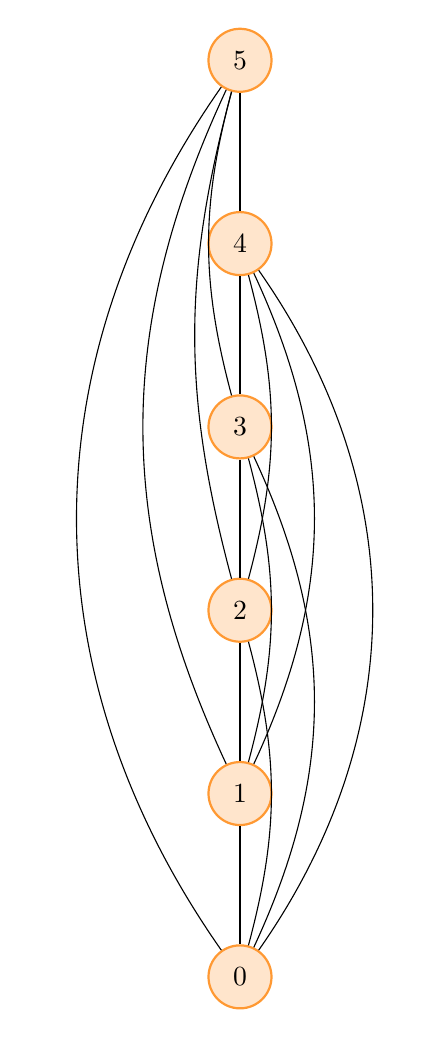
\begin{tikzpicture}[
  node distance=1.5cm,
  every node/.style={circle, draw=orange!80, fill=orange!20, thick, minimum size=8mm},
  arrow/.style={-{Latex[length=2mm]}, thick}
]

% Nodes (top to bottom)
\node(s5) {5};
\node[below=of s5] (s4) {4};
\node[below=of s4] (s3) {3};
\node[below=of s3] (s2) {2};
\node[below=of s2] (s1) {1};
\node[below=of s1] (s0) {0};

% Draw curved undirected edges
\draw (s5) -- (s4);
\draw[bend right=15] (s5) to (s3);
\draw[bend right=15] (s5) to (s2);
\draw[bend right=25] (s5) to (s1);
\draw[bend right=35] (s5) to (s0);

\draw (s4) -- (s3);
\draw[bend left=15] (s4) to (s2);
\draw[bend left=25] (s4) to (s1);
\draw[bend left=35] (s4) to (s0);

\draw (s3) -- (s2);
\draw[bend left=15] (s3) to (s1);
\draw[bend left=25] (s3) to (s0);

\draw (s2) -- (s1);
\draw[bend left=15] (s2) to (s0);

\draw (s1) -- (s0);


\end{tikzpicture}
  \end{solution}
\part[5] Discuss the time complexity of the solution.
  \begin{solution}
    There are $n$ nodes for example and at each node you are looking at all $n-1$ nodes to go to. This effectively gives us $O(n^2)$
  \end{solution}
\part[5] Provide a bottom-up implementation (pseudocode) to compute the minimum stress damage.
  \begin{solution}
    \begin{algorithm}
    Input: Array $a$ of station distances and $n$ which is the number of stations \newline
\caption{MINIMUM-STRESS$(a, n)$}
\begin{algorithmic}[1]
\STATE Let \texttt{minStress}[0..n] be a new array
\STATE \texttt{minStress}[0] $\leftarrow$ 0
\FOR{$j = 1$ to $n$}
    \STATE \texttt{minStress}[j] $\leftarrow \infty$
    \FOR{$i = 0$ to $j-1$}
        \STATE \texttt{cost} $\leftarrow$ \texttt{minStress}[i] $+$ $(1000 - (a[j] - a[i]))^2$
        \IF{\texttt{cost} $<$ \texttt{minStress}[j]}
            \STATE \texttt{minStress}[j] $\leftarrow$ \texttt{cost}
        \ENDIF
    \ENDFOR
\ENDFOR
\RETURN \texttt{minStress}[n]
\end{algorithmic}
\end{algorithm}

  \end{solution}
\part[5] Show how the pseudocode can be modified to also compute the sequence of visited charging stations.
  \begin{solution}
    \begin{algorithm}
    Input: same as before \newline
\caption{MINIMUM-STRESS-AND-SEQUENCE$(a, n)$}
\begin{algorithmic}[1]
\STATE Let \texttt{minStress}[0..n] and \texttt{prev}[0..n] be new arrays
\STATE \texttt{minStress}[0] $\leftarrow$ 0
\STATE \texttt{prev}[0] $\leftarrow$ \texttt{NIL}
\FOR{$j = 1$ to $n$}
    \STATE \texttt{minStress}[j] $\leftarrow \infty$
    \FOR{$i = 0$ to $j-1$}
        \STATE \texttt{cost} $\leftarrow$ \texttt{minStress}[i] $+$ $(1000 - (a[j] - a[i]))^2$
        \IF{\texttt{cost} $<$ \texttt{minStress}[j]}
            \STATE \texttt{minStress}[j] $\leftarrow$ \texttt{cost}
            \STATE \texttt{prev}[j] $\leftarrow$ $i$
        \ENDIF
    \ENDFOR
\ENDFOR

\STATE Initialize empty list \texttt{sequence}
\STATE $k \leftarrow n$
\WHILE{$k \neq$ \texttt{NIL}}
    \STATE Append $k$ to \texttt{sequence}
    \STATE $k \leftarrow$ \texttt{prev}[$k$]
\ENDWHILE
\STATE Reverse \texttt{sequence}
\RETURN \texttt{minStress}[n] and \texttt{sequence}
\end{algorithmic}
\end{algorithm}
  \end{solution}
 
\end{parts}

\end{questions}

\end{document}

%%% Local Variables:
%%% mode: latex
%%% TeX-master: t
%%% End: